\newpage

\captionsetup{labelformat=empty}

\section*{\texorpdfstring{Appendix D: VOI for conservation auctions
heuristic solution \emph{n} =
3}{Appendix D: VOI for conservation auctions heuristic solution n = 3}}\label{appendix-d-voi-for-conservation-auctions-heuristic-solution-n-3}
\addcontentsline{toc}{section}{Appendix D: VOI for conservation auctions
heuristic solution \emph{n} = 3}

\textbf{Priors}

Let \(A_1\), \(A_2\), \(A_3\) be assets. Each has some value \(c_1\),
\(c_2\), and \(c_3\) which are uncertain with a joint prior probability
distribution,

\begin{equation}
\begin{bmatrix}c_1 \\ c_2 \\ c_3\end{bmatrix}\sim\mathcal{N}\left(\begin{bmatrix}\mu_1 \\ \mu_2 \\ \mu_3\end{bmatrix}, \begin{bmatrix}\sigma^2_1 & 0 & 0 \\ 0 & \sigma^2_2 & 0\\ 0 & 0 & \sigma^2_3 \end{bmatrix}\right)
(\#eq:jointprior)
\end{equation}

where \(\mu_1\), \(\mu_2\), and \(\mu_3\) are means and \(\sigma_1\),
\(\sigma_2\) and \(\sigma_3\) are the prior standard deviations.

\textbf{Utilities}

We assign utilities to each rank order of \(c_1\), \(c_2\), and \(c_3\)
in combination with each action of purchasing one of \(A\), \(B\) or
\(C\),

\begin{equation}
\begin{aligned}
u(A_1, c_1 > c_2 > c_3)&=1\\
u(A_1, c_1 > c_3 > c_2)&=1\\
u(A_1, c_2 > c_1 > c_3)&=0.5\\
u(A_1, c_3 > c_1 > c_2)&=0.5\\
u(A_1, c_2 > c_3 > c_1)&=0\\
u(A_1, c_3 > c_2 > c_1)&=0\\
u(A_2, c_2 > c_1 > c_3)&=1\\
\mathrm{etc...}&
\end{aligned}
(\#eq:utilitiesapen2)
\end{equation}

such that utility is maximised when we purchase the highest ranked
asset, zero when we purchase the lowest ranked and somewhere inbetween
when we purchase the middle ranked asset.

\textbf{Ranking probabilties}

We can express the probability of any assets being in a given rank order
as the probabililty of two differences being less than zero. Such that,
for example,

\begin{equation}
\Pr(c_1 > c_2 > c_3) = \Pr(c_2 - c_1 < 0,  c_3 - c_2 < 0)
(\#eq:probrankapen)
\end{equation}

Given this we define two new variables, \(z_1\) and \(z_2\) where

\begin{equation}
\begin{aligned}
  z_1 &= c_2 - c_1,\\
  z_2 &= c_3 - c_2
\end{aligned}
(\#eq:z12apen)
\end{equation}

Even if \(c_1\), \(c_2\), and \(c_3\) are all uncorrelated \(z_1\) and
\(z_2\) will not be, where

\begin{equation}
\mathrm{cov}(z_1, z_2)=\mathrm{cov}(c_1, c_2) - \mathrm{var}(c_2) - \mathrm{cov}(c_1, c_3) + \mathrm{cov}(c_2, c_3)
(\#eq:covz)
\end{equation}

Which, when \(c_1\), \(c_2\), and \(c_3\) are all uncorrelated
simplifies to

\begin{equation}
\mathrm{cov}(z_1, z_2)=-\mathrm{var}(c_2)
(\#eq:covz2)
\end{equation}

Therefore the joint distribution of \(z_1\) and \(z_2\) is,

\begin{equation}
\begin{bmatrix}z_1\\z_2\end{bmatrix}
  \sim\mathrm{N}\left(
  \begin{bmatrix}\mu_2-\mu_1\\\mu_3-\mu_2\end{bmatrix},
  \begin{bmatrix}\sigma^2_1+\sigma^2_2&-\sigma^2_2\\-\sigma^2_2&\sigma^2_2+\sigma^2_3\end{bmatrix}\right)
(\#eq:jointzapen)
\end{equation}

To obtain \(\Pr(c_1 > c_2 > c_3)\) we evalute the multivariate
cumulative distribution function of \(z_1\) and \(z_2\),

\begin{equation}
\Phi(z_1,z_2)
(\#eq:phiz)
\end{equation}

within the limits, \(-\infty\) and 0.

\textbf{Expected value of perfect information}

To calculate the prior expected utility of purchasing any asset, we
weight the utilities for that action (eqn. 2) by the relevant
probablities calculated from eqns. 3--9. For instance;

\begin{equation}
\begin{aligned}
  \mathrm{E}[u(A_1)] = & 1 \times \Pr(c_1 > c_2 > c_3) + 1 \times \Pr(c_1 > c_3 > c_2)\,+ \\
  &0.5 \times \Pr(c_2 > c_1 > c_3) + 0.5 \times \Pr(c_3 > c_1 > c_2)\,+ \\
  &0 \times \Pr(c_2 > c_3 > c_1) + 0 \times \Pr(c_3 > c_2 > c_1)
\end{aligned}
(\#eq:EuA1apen)
\end{equation}

The expected value of perfect information then is,

\begin{equation}
\mathrm{EVPI}=1-\max(\mathrm{E}[u(A_1)],\mathrm{E}[u(A_2)],\mathrm{E}[u(A_3)])
(\#eq:evpiapen2)
\end{equation}

\textbf{Updating}

Now suppose we can update the priors for \(c_1\), \(c_2\), and \(c_3\)
by taking \(M\) samples from sampling distrubutions with, for
simplicity, some fixed variance of 1 and centered on \(\mu_1\),
\(\mu_2\) and \(\mu_3\) respectively. Further, we can define \(p_1\) and
\(p_2\) as the proportion of the \(M\) samples allocated to sampling for
\(A_1\) and \(A_2\) respectively with \(1 - p_1 - p_2\) being allocated
to \(A_3\). We can then use these samples to update the priors for
\(c_1\), \(c_2\), and \(c_3\) to obtain preposterior estimates,
\(c^\prime_1\), \(c^\prime_2\), and \(c^\prime_3\), where,

\begin{equation}
\begin{bmatrix}c^\prime_1 \\ c^\prime_2 \\ c^\prime_3\end{bmatrix}\sim\mathcal{N}\left(\begin{bmatrix}\mu_1 \\ \mu_2 \\ \mu_3\end{bmatrix}, \begin{bmatrix}\frac{\sigma^2_1}{Mp_1\sigma^2_1 + 1} & 0 & 0 \\ 0 & \frac{\sigma^2_2}{Mp_2\sigma^2_2 + 1} & 0\\ 0 & 0 & \frac{\sigma^2_3}{M(1 - p_1 - p_2)\sigma^2_3 + 1} \end{bmatrix}\right)
(\#eq:jointpost)
\end{equation}

\textbf{Expected value of sample information}

For any given new rank order, based on the updated preposterior
distributions, we can again calculate a probablity by defining new
variables (i.e., \(z^\prime_1\) and \(z^\prime_2\)) and evalute their
multivariate cumulative distribution as in eqns. 3--9. Therefore we can
obtain the preposterior expected utilities for each purchase action by
weighting the preposterior probablites by their respective utilities as
in eqn. 10. Accordingly the expected vale of sample information is

\begin{equation}
\mathrm{EVSI}=\max(\mathrm{E}^\prime[u(A_1)],\mathrm{E}^\prime[u(A_2)],\mathrm{E}^\prime[u(A_3)])-\max(\mathrm{E}[u(A_1)],\mathrm{E}[u(A_2)],\mathrm{E}[u(A_3)])
(\#eq:evsiapen2)
\end{equation}

\textbf{Optimisation}

Using eqns 8-13 we can find the optimal values of \(p_1\) and \(p_2\)
for any given \(M\) that will maximise the EVSI. Below we examine a
number of \_\_Case studies for different sets of prior distrbutions for
\(c_1\), \(c_2\) and \(c_3\).

\textbf{Summary}

\begin{itemize}
\tightlist
\item
  Optimal allocation sensitive to ratios of \(\mu\)'s.
\item
  Optimal allocation sensitive to ratio of \(\sigma\)'s.
\item
  Not always preferential to sample asset with greater uncertainty.
\item
  Solution is symmetrical.
\end{itemize}

\textbf{Case study 1: homogenous prior \(\sigma\)'s and homogenous prior
means}

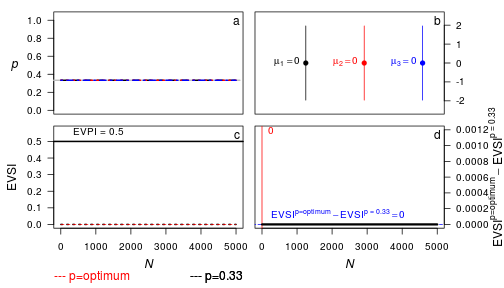
\includegraphics{figure/x000_1_1_1-1.png} \clearpage

\textbf{Case study 2a: homogenous prior \(\sigma\)'s and heterogenous
prior means}

\(\mu_1 = \mu_2 > \mu_3\)

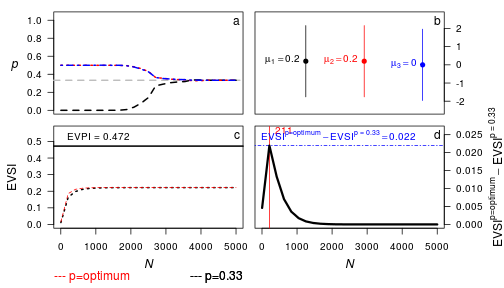
\includegraphics{figure/x110_1_1_1c-1.png} \clearpage

\textbf{Case study 2b: homogenous prior \(\sigma\)'s and heterogenous
prior means}

\(\mu_1 > \mu_2 = \mu_3\)

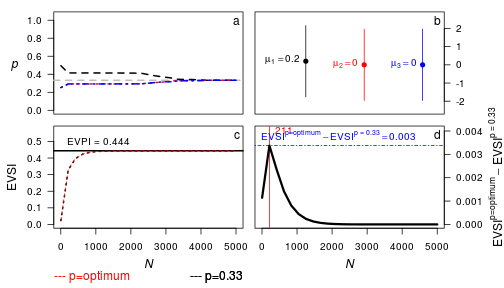
\includegraphics{figure/x100_1_1_1c-1.png} \clearpage

\textbf{Case study 2c: homogenous prior \(\sigma\)'s and heterogenous
prior means}

\(\mu_1 > \mu_2 > \mu_3\)

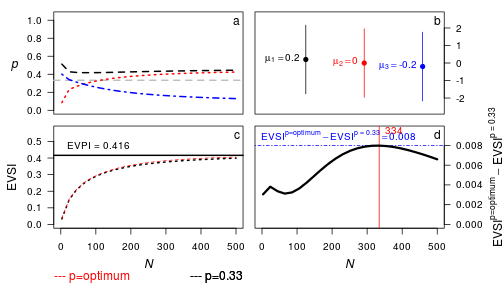
\includegraphics{figure/x10n1_1_1_1c-1.png} \clearpage

\textbf{Case study 3a: heterogenous prior \(\sigma\)'s and heterogenous
prior means}

\(\mu_1 > \mu_2 = \mu_3\)

\(\sigma_1 > \sigma_2 = \sigma_3\)

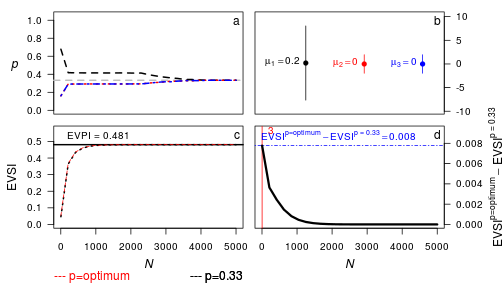
\includegraphics{figure/x100___1_1_1c-1.png} \clearpage

\textbf{Case study 3b: heterogenous prior \(\sigma\)'s and heterogenous
prior means}

\(\mu_1 > \mu_2 = \mu_3\)

\(\sigma_1 < \sigma_2 = \sigma_3\)

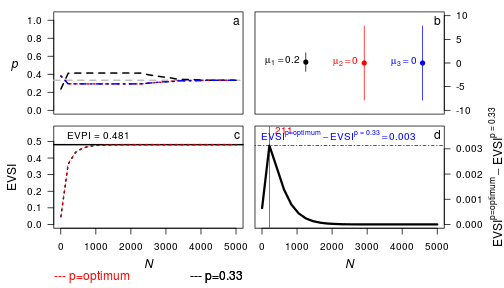
\includegraphics{figure/x1001_1_1c-1.png} \clearpage

\textbf{Case study 3c: heterogenous prior \(\sigma\)'s and heterogenous
prior means}

\(\mu_1 = \mu_2 > \mu_3\)

\(\sigma_1 = \sigma_2 < \sigma_3\)

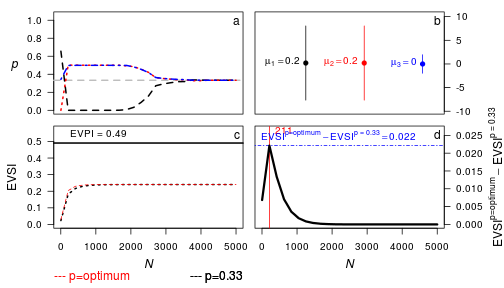
\includegraphics{figure/x110__1__1_1c-1.png} \clearpage

\textbf{Case study 3d: heterogenous prior \(\sigma\)'s and heterogenous
prior means}

\(\mu_1 > \mu_2 = \mu_3\)

\(\sigma_1 = \sigma_2 > \sigma_3\)

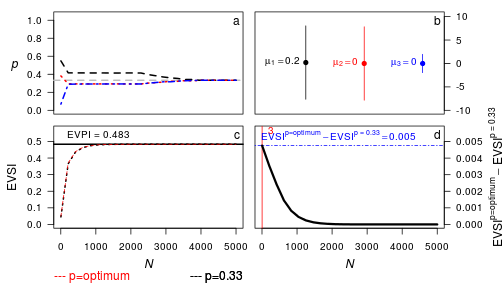
\includegraphics{figure/x100__1__1_1c-1.png} \clearpage

\textbf{Case study 3e: heterogenous prior \(\sigma\)'s and heterogenous
prior means}

\(\mu_1 > \mu_2 = \mu_3\)

\(\sigma_1 = \sigma_2 < \sigma_3\)

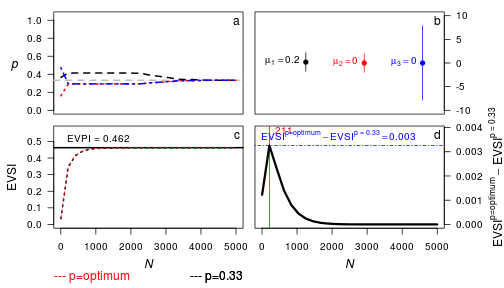
\includegraphics{figure/x100_1_1__1c-1.png} \clearpage

\textbf{Case study 3f: heterogenous prior \(\sigma\)'s and heterogenous
prior means}

\(\mu_1 = \mu_2 > \mu_3\)

\(\sigma_1 = \sigma_3 > \sigma_2\)

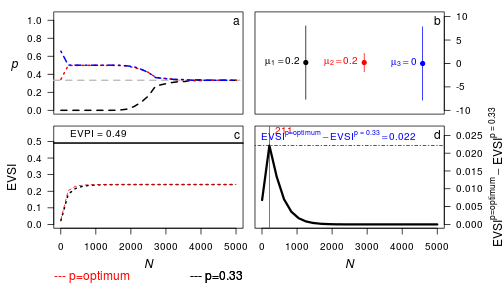
\includegraphics{figure/x110__1_1__1c-1.png} \clearpage

\textbf{Case study 3g: heterogenous prior \(\sigma\)'s and heterogenous
prior means}

\(\mu_1 = \mu_2 > \mu_3\)

\(\sigma_1 = \sigma_3 < \sigma_2\)

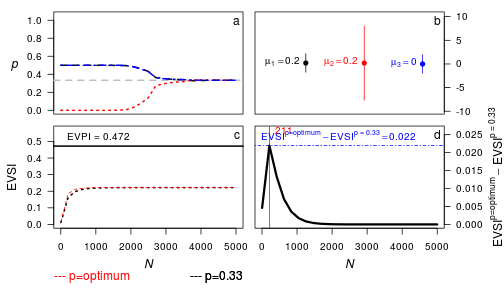
\includegraphics{figure/x110_1__1_1c-1.png} \clearpage

\textbf{Case study 3h: heterogenous prior \(\sigma\)'s and heterogenous
prior means}

\(\mu_1 > \mu_2 = \mu_3\)

\(\sigma_1 < \sigma_2 < \sigma_3\)

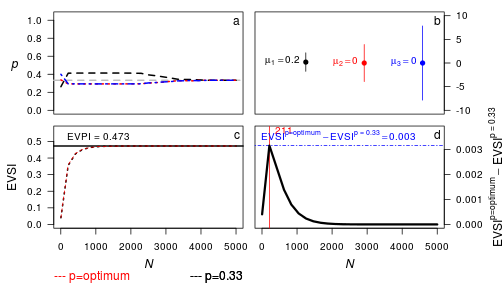
\includegraphics{figure/x100_1__1___1c-1.png} \clearpage  

\textbf{Case study 3i: heterogenous prior \(\sigma\)'s and heterogenous
prior means}

\(\mu_1 > \mu_2 = \mu_3\)

\(\sigma_2 < \sigma_1 < \sigma_3\)

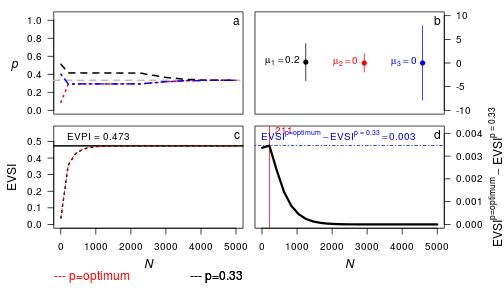
\includegraphics{figure/x100__1_1___1c-1.png} \clearpage

\textbf{Case study 3j: heterogenous prior \(\sigma\)'s and heterogenous
prior means}

\(\mu_1 > \mu_2 = \mu_3\)

\(\sigma_1 > \sigma_2 > \sigma_3\)

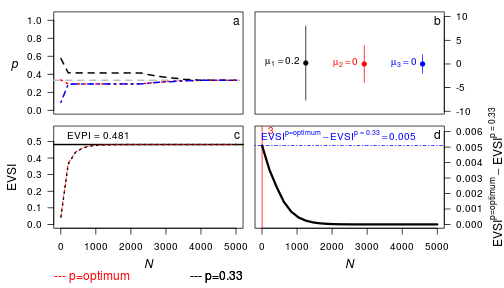
\includegraphics{figure/x100___1__1_1c-1.png} \clearpage

\textbf{Case study 3k: heterogenous prior \(\sigma\)'s and heterogenous
prior means}

\(\mu_1 = \mu_2 > \mu_3\)

\(\sigma_1 < \sigma_2 < \sigma_3\)

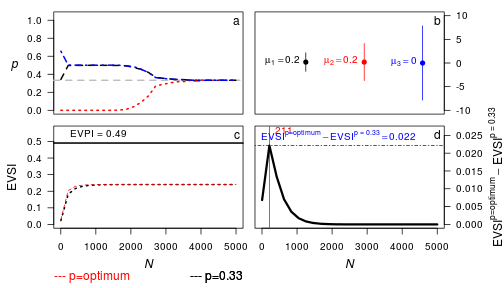
\includegraphics{figure/x110_1__1___1c-1.png} \clearpage

\textbf{Case study 3l: heterogenous prior \(\sigma\)'s and heterogenous
prior means}

\(\mu_1 = \mu_2 > \mu_3\)

\(\sigma_1 < \sigma_3 < \sigma_2\)

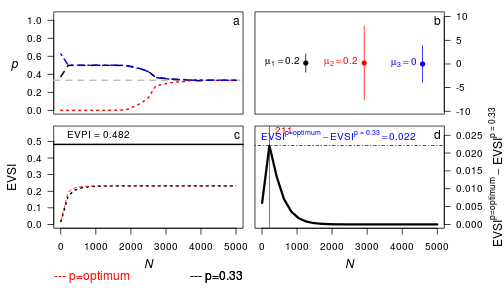
\includegraphics{figure/x110_1___1__1c-1.png} \clearpage  

\textbf{Case study 3m: heterogenous prior \(\sigma\)'s and heterogenous
prior means}

\(\mu_1 = \mu_2 > \mu_3\)

\(\sigma_1 > \sigma_2 > \sigma_3\)

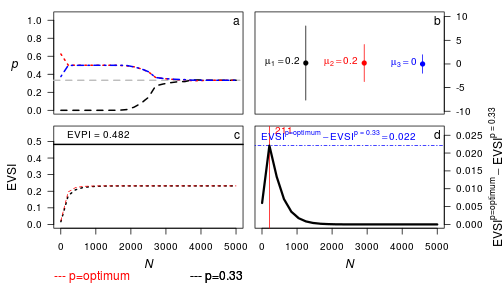
\includegraphics{figure/x110___1__1_1c-1.png} \clearpage

\textbf{Case study 3n: heterogenous prior \(\sigma\)'s and heterogenous
prior means}

\(\mu_1 > \mu_2 > \mu_3\)

\(\sigma_1 < \sigma_2 = \sigma_3\)

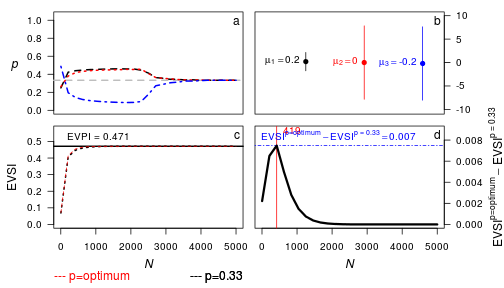
\includegraphics{figure/x10n1_1__1__1c-1.png} \clearpage

\textbf{Case study 3o: heterogenous prior \(\sigma\)'s and heterogenous
prior means}

\(\mu_1 > \mu_2 > \mu_3\)

\(\sigma_1 = \sigma_2 < \sigma_3\)

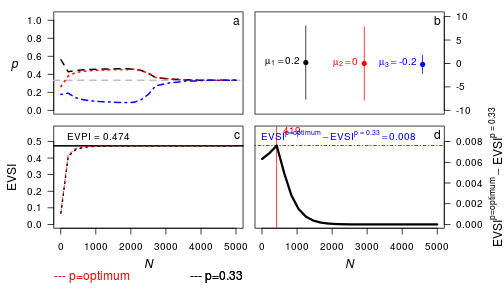
\includegraphics{figure/x10n1__1__1_1c-1.png} \clearpage

\textbf{Case study 3p: heterogenous prior \(\sigma\)'s and heterogenous
prior means}

\(\mu_1 > \mu_2 > \mu_3\)

\(\sigma_1 = \sigma_3 > \sigma_2\)

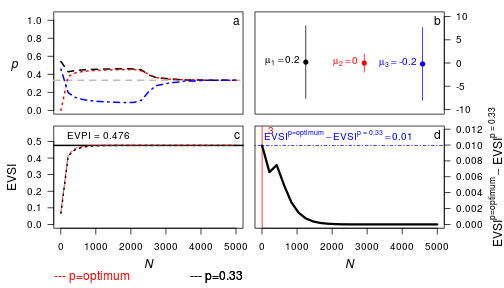
\includegraphics{figure/x10n1__1_1__1c-1.png} \clearpage  

\textbf{Case study 3q: heterogenous prior \(\sigma\)'s and heterogenous
prior means}

\(\mu_1 > \mu_2 > \mu_3\)

\(\sigma_1 = \sigma_2 < \sigma_3\)

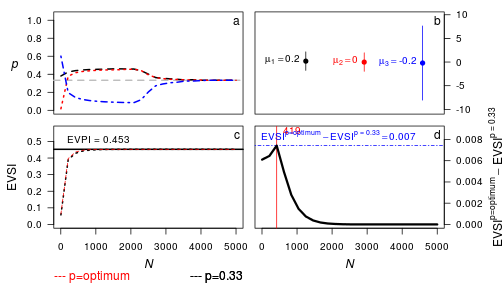
\includegraphics{figure/x10n1_1_1__1c-1.png} \clearpage

\textbf{Case study 3r: heterogenous prior \(\sigma\)'s and heterogenous
prior means}

\(\mu_1 > \mu_2 > \mu_3\)

\(\sigma_1 > \sigma_2 = \sigma_3\)

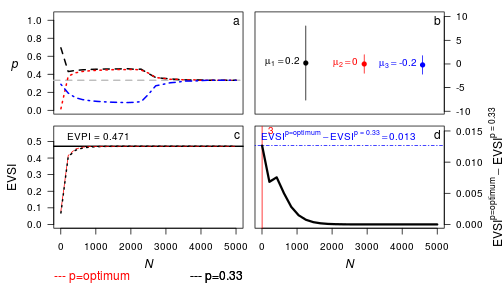
\includegraphics{figure/x10n1__1_1_1c-1.png} \clearpage

\textbf{Case study 3s: heterogenous prior \(\sigma\)'s and heterogenous
prior means}

\(\mu_1 > \mu_2 > \mu_3\)

\(\sigma_1 = \sigma_3 < \sigma_2\)

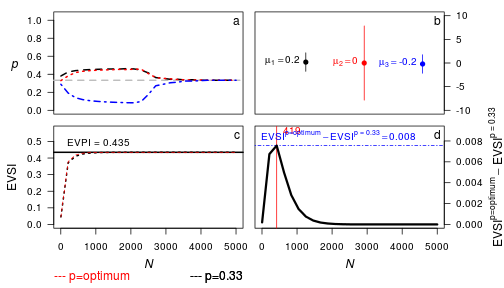
\includegraphics{figure/x10n1_1__1_1c-1.png} \clearpage

\textbf{Case study 3t: heterogenous prior \(\sigma\)'s and heterogenous
prior means}

\(\mu_1 > \mu_2 > \mu_3\)

\(\sigma_1 < \sigma_2 < \sigma_3\)

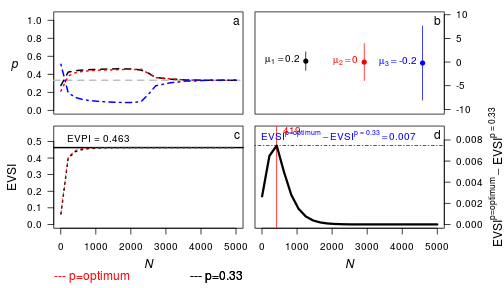
\includegraphics{figure/x10n1_1__1___1c-1.png} \clearpage  

\textbf{Case study 3u: heterogenous prior \(\sigma\)'s and heterogenous
prior means}

\(\mu_1 > \mu_2 > \mu_3\)

\(\sigma_2 < \sigma_1 < \sigma_3\)

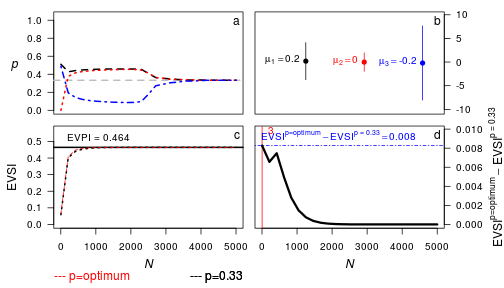
\includegraphics{figure/x10n1__1_1___1c-1.png} \clearpage

\textbf{Case study 3v: heterogenous prior \(\sigma\)'s and heterogenous
prior means}

\(\mu_1 > \mu_2 > \mu_3\)

\(\sigma_1 < \sigma_3 < \sigma_2\)

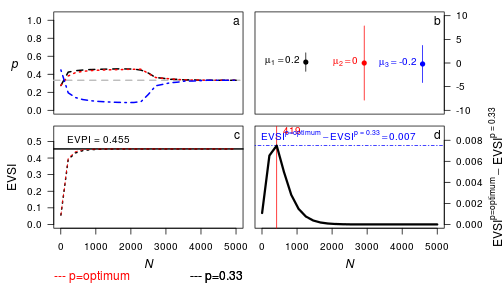
\includegraphics{figure/x10n1_1___1__1c-1.png} \clearpage

\textbf{Case study 3w: heterogenous prior \(\sigma\)'s and heterogenous
prior means}

\(\mu_1 > \mu_2 > \mu_3\)

\(\sigma_1 > \sigma_3 > \sigma_2\)

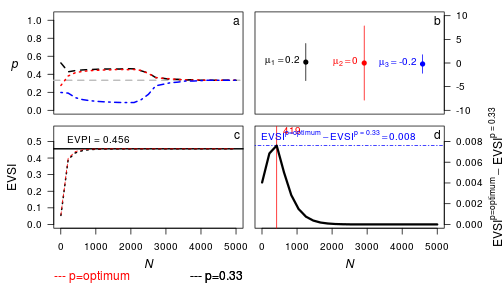
\includegraphics{figure/x10n1__1___1_1c-1.png} \clearpage

\textbf{Case study 3x: heterogenous prior \(\sigma\)'s and heterogenous
prior means}

\(\mu_1 > \mu_2 > \mu_3\)

\(\sigma_1 > \sigma_2 > \sigma_3\)

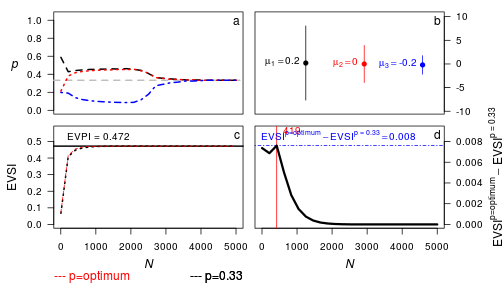
\includegraphics{figure/x10n1___1__1_1c-1.png} \clearpage

\captionsetup{labelformat=default}
